\section{IMU-based Approaches: Passive Phase Suppression}

% comment: add image quality evaluation?

\begin{figure}[h]
\begin{center}
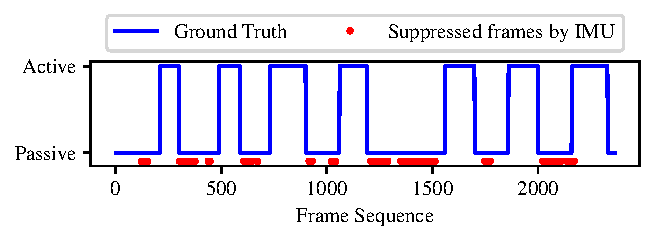
\includegraphics[width=.9\linewidth]{FIGS/fig-imu-trace-lego.pdf}\\
{\small (a) LEGO}
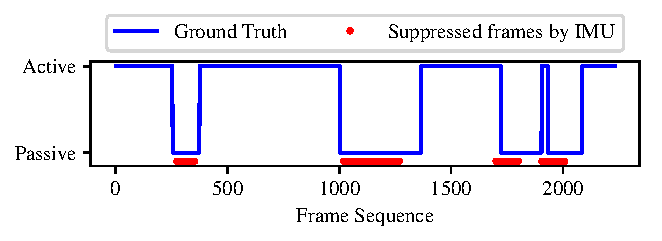
\includegraphics[width=.9\linewidth]{FIGS/fig-imu-trace-pingpong.pdf}\\
{\small (b) PING PONG}
\end{center}
\vspace{-0.1in}
\caption{\small Accuracy of IMU-based Frame Suppression}
\label{fig:imu-trace-example}
\vspace{-0.1in}
\end{figure}

In many applications, passive phases can often be associated with the user's
head movement. We illustrate with two applications here. In LEGO, during the
passive phase, which begins after the user receives the next instruction, a user
typically turns away from the LEGO board and starts searching for the next brick
to use in a parts box. During this period, the computer vision algorithm would
detect no meaningful task states if the frames are transmitted.  In PING PONG
application (Section~\ref{sec:example-apps}), an active phase lasts
throughout a rally.  Passive phases are in between actual game play, when the
user takes a drink, switches sides, or, most commonly, tracks down and picks up
a wayward ball from the floor. These are associated with much large range of
head movements than during a rally when the player generally looks toward the
opposing player.  Again, the frames can be suppressed on the client to reduce
wireless transmission and load on the cloudlet.  In both scenarios, significant
body movement can be detected through Inertial Measurement Unit (IMU) readings
on the wearable device, and used to predict those passive phases.

For each frame, we get a six-dimensional reading from the IMU:
rotation in three axes, and acceleration in three axes.  We train an
application-specific SVM to predict active/passive phases based on IMU
readings, and suppress predicted passive frames on the client.
Figure~\ref{fig:imu-trace-example}(a) and (b) show an example trace
from LEGO and PING PONG, respectively.  Human-labeled ground truth
indicating passive and active phases is shown in blue.  The red dots
indicate predictions of passive phase frames based on the IMU
readings; these frames are suppressed at the client and not
transmitted.  Note that in both traces, the suppressed frames also
form streaks. In other words, a number of frames in a row can be
suppressed. As a result, the saving we gain from IMU is orthogonal to
that from adaptive sampling.

Although the IMU approach does not capture all of the passive frames
(e.g., in LEGO, the user may hold his head steady while looking for
the next part), when a passive frame is predicted, this is likely
correct (i.e., high precision, moderate recall).  Thus, we expect
little impact on event detection accuracy or latency, as few if any
active phase frames are affected.  This is confirmed in
Table~\ref{tab:imu-result}, which summarizes results for five traces
from each application.  We are able to suppress up to 49.9\% of
passive frames for LEGO and up to 38.4\% of passive frames in case of
PING PONG on the client, while having minimal impact on application
quality --- incurring no delay in state change detection in LEGO, and
less than 2\% loss of active frames in PING PONG.

\begin{table}[h]
\small\centering
\begin{tabular}{| l | c | c |}
   \hline
        & Suppressed  &  Max Delay of \\ 
        & Passive Frames (\%)   & State Change Detection \\ \hline
    Trace 1 & 17.9\%    & 0 \\
    Trace 2 & 49.9\%    & 0 \\
    Trace 3 & 27.1\%    & 0 \\
    Trace 4 & 37.0\%    & 0 \\
    Trace 5 & 34.1\%    & 0 \\
    \hline
\end{tabular}\\[0.1in]
{\small (a) LEGO}\\[0.1in]

\begin{tabular}{| l | c | c |}
    \hline
        & Suppressed        & Loss of  \\
        & Passive Frames (\%)    & Active Frames (\%) \\ \hline
    Trace 1 & 21.5\%    &   0.8\%   \\
    Trace 2 & 30.0\%    &   1.5\%   \\
    Trace 3 & 26.2\%    &   1.9\%   \\
    Trace 4 & 29.8\%    &   1.0\%   \\
    Trace 5 & 38.4\%    &   0.2\%   \\
    \hline
\end{tabular}\\[0.1in]
{\small (b) PING PONG}\\[0.1in]
\caption{\small Effectiveness of IMU-based Frame Suppression}
\label{tab:imu-result}
\end{table}
